\documentclass[a4paper, 11pt]{article}

\usepackage{graphicx}


\usepackage{wrapfig}
\usepackage{lipsum}

\usepackage[utf8]{inputenc}

\usepackage{mathpazo} % Use the Palatino font
\usepackage[T1]{fontenc} % Required for accented characters
\linespread{1.05} % Change line spacing here, Palatino benefits from a slight increase by default

\usepackage{float}
\usepackage{hyperref}
\hypersetup{
	colorlinks=true, 		% Aktivieren von farbigen Links im Dokument
	linkcolor=blue, 	% Farbe festlegen
	urlcolor=blue,
	linktocpage=true, 		% Nicht der Text sondern die Seitenzahlen in Verzeichnissen klickbar
	bookmarksnumbered=true 	% Überschriftsnummerierung im PDF Inhalt anzeigen.
}
\usepackage{eurosym}
\usepackage[ngerman]{babel}
\usepackage{tabularx}
\usepackage[table,xcdraw]{xcolor}
\usepackage{color}
 
\definecolor{pblue}{rgb}{0.13,0.13,1}
\definecolor{pgreen}{rgb}{0,0.5,0}
\definecolor{pred}{rgb}{0.9,0,0}
\definecolor{pgrey}{rgb}{0.46,0.45,0.48}

\usepackage{listings}
\lstset{language=Java,
  showspaces=false,
  showtabs=false,
  breaklines=true,
  showstringspaces=false,
  breakatwhitespace=true,
  commentstyle=\color{pgreen},
  keywordstyle=\color{pblue},
  stringstyle=\color{pred},
  basicstyle=\ttfamily,
  moredelim=[il][\textcolor{pgrey}]{$$},
  moredelim=[is][\textcolor{pgrey}]{\%\%}{\%\%}
}

\makeatletter

\renewcommand{\maketitle}{ % Customize the title - do not edit title and author name here, see the TITLE block below
\begin{flushright} % Right align
{\LARGE\@title} % Increase the font size of the title

\vspace{10pt} % Some vertical space between the title and author name

{\large\@author} % Author name
\\\@date % Date

\vspace{20pt} % Some vertical space between the author block and abstract
\end{flushright}
}


\providecommand{\tightlist}{%
  \setlength{\itemsep}{0pt}\setlength{\parskip}{0pt}}

\title{\textbf{Arbeitsdokumentation des Backendteam}} 

\author{Team Backend} 

\date{\today} % Date

\begin{document}
\renewcommand{\@listI}{\itemsep=0pt} % Reduce the space between items in the itemize and enumerate environments and the bibliography

\maketitle % Print the title section

Die Umsetzung der in der API-Spec definierten Funktionalität erfolgt im
Backend. Dies ist eine Java-Applikation, welche auf einem
Tomcat-Appli\-ka\-tions\-server läuft. Die Applikation übernimmt unter anderem
folgende Aufgaben:

\begin{itemize}
    \tightlist
    \item Bereitstellen der API-Routen
    \item Abbilden der Businesslogik
    \item Speichern in einer Datenbank
    \item Authentifizierung und Authorisierung
\end{itemize}

\section{Einstieg in Spring Boot}

Die Entwicklung erfolgt mithilfe des Frameworks
\href{https://en.wikipedia.org/wiki/Spring_Boot#Spring_Boot}{Spring Boot}. Das
Framework bietet verschiedene Features, die die Entwicklung erleichtern oder
strukturieren. Es ist zum Beispiel möglich, einen
\href{https://de.wikipedia.org/wiki/Objektrelationale_Abbildung}{objektrelationalen
Mapper}
zu nutzen, der den Datenbankzugriff stark abstrahiert. Auch das Bereitstellen
der API-Routen wird durch Spring Boot vereinfacht. Zusätzlich hat das
Framework eine gewissen \emph{Meinung}, mit welchen Mustern entwickelt werden
soll, welches sehr hilfreich für uns unerfahrene Entwickler war.

Zum Einstieg in das Backend-Projekt und dem Kennenlernen der Spring Boot-Basics
betrachten wir die Flugzeugverwaltung. Die findet im Paket \lstinline{Plane}
statt, in dem zwei Klassen und ein Interface definiert werden (vgl. Abbildung
\ref{fig:planes_package}).

\begin{figure}[htpb]
    \centering
    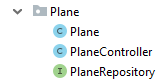
\includegraphics{images/plane_package.png}
    \caption{Inhalt des Package \lstinline{Plane}}
    \label{fig:planes_package}
\end{figure}

Dabei ist die Klasse \lstinline{Plane} das Business-Objekt, welches ein Flugzeug
repräsentiert. Im \lstinline{PlaneController} werden die Webservice-Routen und die
Business-Logik definiert und das \lstinline{PlaneRepository} abstrahiert das
Speichern von \lstinline{Plane}-Objekten in der Datenbank.

Schauen wir uns nun zunächst einen Ausschnitt aus der \lstinline{Plane}-Klasse an:

\begin{lstlisting}[caption=Entity-Klasse]
@Entity
public class Plane {

    @Id
    @GeneratedValue(strategy = GenerationType.IDENTITY)
    private Integer id;
    private String number;
    private String name;
    ...
}
\end{lstlisting}

Die \lstinline{@Entity}-Annotation gibt an, dass die Klasse in der Datenbank
gespeichert werden soll, wobei die \lstinline{id} der Primärschlüssel hierfür
ist und vom Framework generiert werden soll.

\begin{figure}[htpb]
    \centering
    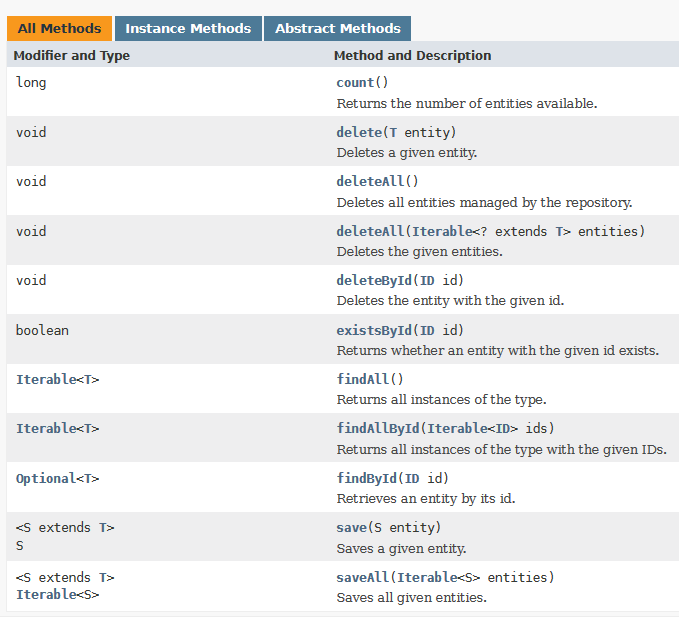
\includegraphics[width=\textwidth]{images/crudrepository.png}
    \caption{Ausschnitt der Methoden, die das PlaneRepository bereitstellt}
    \label{fig:crudrepository}
\end{figure}

Das \texttt{PlaneRepository} verwaltet dann die Datenbank-Interaktion und
stellt dafür unter anderem die Methoden aus Abbildung \ref{fig:crudrepository}
bereit. Diese Methoden erbt es von einem Interface, welches aus dem
Spring-Framework kommt. Daher wird der Datenbankzugriff in der Entwicklung
stark vereinfacht. Es ist an keiner Stelle nötig, SQL-Befehle zu formulieren.
Auch Schemata werden automatisch generiert. Dies ist ein besonders großer
Vorteil, da so eine Änderung in der Java-Klasse automatisch im Datenbankschema
übernommen wird. 

\begin{figure}[htpb]
    \centering
    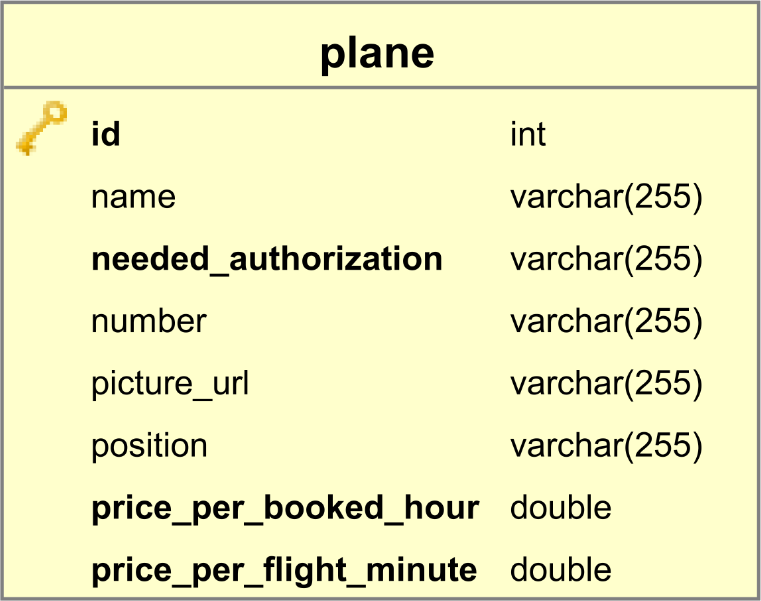
\includegraphics[width=0.4\textwidth]{images/erm/plane.png}
    \caption{Generierte Tabelle, die \texttt{Plane}-Objekte speichert}
    \label{fig:plane_table}
\end{figure}

Abbildung \ref{fig:plane_table} zeigt die MySQL-Tabelle, die vom
objekt-relationalen Mapper generiert wurde, um die \texttt{Plane}-Objekte zu
persitieren. Diese Tabelle wird automatisch durch die Entity-Annotation
erstellt. Wenn sich die Klasse verändert, wird auch beim nächsten Start der
Applikation auch die Tabelle geändert. Durch diese Abstraktion wird ein
hypothetisches Datenbank-Team in der Entwicklung unnötig, da nur noch zu
Kontroll- und Test-Zwecken direkt auf die Datenbank zugegriffen wird.


\begin{lstlisting}[caption=Ausschnitt eines REST-Controllers, label=lst_controller, float]
@RestController
@RequestMapping(path = "planes")
public class PlaneController {
...
    @GetMapping(path = "/{id}")
    public Plane detail(@PathVariable int id) {

    return planeRepository.findById(id)
            .orElseThrow(() -> new NoSuchElementException();
    }
...
}
\end{lstlisting}


Der \texttt{PlaneController} enthält nun die Business-Logik.  In Listing
\ref{lst_controller} wird die Definition der unter dem Pfad
\url{<server>:<port>/planes/{id}} anzufindengen Methode gezeigt. Es wird in der
URL also als Parameter angegeben, welches Flugzeug angezeigt werden soll, woraufhin
das Flugzeug in der Datenbank gesucht wird. Wird es gefunden, wird es
zurückgegeben, wird kein Flugzeug gefunden, wird eine \lstinline{Exception}
geworfen. Hierbei übernimmt Spring Boot, oder genauer, die Bibliothek \emph{Jackson}
das \emph{Marshalling} und \emph{Unmarshalling}, also das Umwandeln von JSON zu
einfachen Java-Objekten und umgekehrt. 

Dieser Dreiklang aus Business-Objekt, dazugehörigem Controller und Repository
ist relativ typisch für die meisten Business-Objekte im Projekt.

\section{Die Business-Objekte und -Logik}

\subsection{Relationen mit Hibernate}

Eine Übersicht über die Business-Objekte des Projekts kann das Diagramm in
Abbildung \ref{fig:erm_all} geben. Es wurde aus den Datenbanktabellen
generiert, welche wiederum mit \emph{Hibernate}, dem objekt-relationalen
Mapper, generiert wurden.

Relationen zwischen Objekten/Entitäten werden im Quellcode über Annotationen
wie \lstinline{@OneToOne}, \lstinline{@OneToManty} und \lstinline{@ManyToMany}
zwischen den Objekten abgebildet. Listing \ref{lst_relation} zeigt einen
Ausschnitt der Member-Klasse, die das zentrale Business-Objekt ist, welches ein
Vereinsmitglied abbildet. Ein Vereinsmitglied hat unter anderem ein Logbuch,
abgebildet als \lstinline{pilotLog}, für seine Flüge und eine Reihe von
Berechtigungen und Lizenzen, wie zum Beispiel die Privatpilotenlizenz,
abgebildet als eine Liste von \lstinline{flightAuthorization}-Objekten.

Alle diese Objekte sind \emph{Hibernate}-Entitäten. Dadurch werden
entsprechende Tabellen in der Datenbank angelegt. Durch die Annotationen werden
nun die Relationen charakterisiert. Der Parameter \lstinline{cascade = CascadeType.ALL} gibt an, dass wenn ein \lstinline{Member} über das
\lstinline{MemberRepository}, welches sich analog dem
\lstinline{PlaneRepository} verhält, aus der Datenbank geladen werden soll,
auch gleich das Objekt, mit dem der Member in Relation steht, mitgeladen werden
soll.

\begin{lstlisting}[caption=Verknüpfung zu anderen Entitäten in der Member-Klasse,label=lst_relation]
@OneToMany(cascade = CascadeType.ALL)
private List<FlightAuthorization> flightAuthorization = new ArrayList<>();

@OneToOne(cascade = CascadeType.ALL)
private PilotLog pilotLog;
\end{lstlisting}

\begin{figure}[htpb]
    \centering
    \includegraphics[width=\textwidth]{images/erm/all_orthogonal.png}
    \caption{Diagramm des Datenbanktabellen}
    \label{fig:erm_all}
\end{figure}

\subsection{Vereinskonto}

Während der Member ein schönes Beispiel ist, wie relativ typische Sachverhalte
mit Hibernate umgesetzt werden können, ist das \emph{Vereinskonto} ein Beispiel
für eine Stelle , an der wir etwas kreativer werden mussten im Umgang mit
dieser Technologie.

Die Mitglieder besitzen ein Mitgliedskonto, in dem ihre Transaktionen, \emph{zum
Beispiel das Zahlen der Mitgliedsgebühr und ihr Kontostand,} verwaltet werden.
Auch der Verein hat so ein Konto. Hier wird es nun schwierig: Die
Mitgliederkonten sind Objekte, die Mitgliedern zugeordnet sind. Wie also das
Vereinskonto gestalten? Es wurden zwei Vorschläge diskutiert:

\begin{itemize}
    \item Das Vereinskonto ist von einer anderen Klasse als das Mitgliedskonto
        und ein \emph{Singleton}.
    \item ein \emph{unsichtbares} Mitglied repäsentiert den Verein und dessen
        Konto ist das Vereinskonto.
\end{itemize}

Die Umsetzung des Vereinskontos als Singleton, eine Klasse, von der immer
maximal eine Instanz existiert, scheint logisch. Der zweite Vorschlag wurde
formuliert, falls sich der erste als nicht umsetzbar erweist, mangelt aber der
Eleganz des ersten.

Bei der Implementierung des Vereinskontos als Singleton gab es Hürden:

Das Konto sollte vom Mitgliedskonto erben, mit den zwei Unterschieden, dass es
zum einen ein Singleton ist und zum anderen andere Transaktionen speichert. Das
ganze lies sich implementieren, wenn auch mit einigem Aufwand und einem
zwischenzeitlichen versteckten Bug, der eine halbe Woche später gefunden wurde
und über einige Tage aufwändig analysiert werden musste. Hier war
\emph{Hibernate} an einigen Stellen eher eine Herausforderunge als eine Hilfe.

\subsection{Transactions}

In den Konten werden verschiedene Transaktionen gespeichert. Grundsätzlich gibt es aus Vereinssicht zwei Typen von Transaktionen:

\begin{itemize}
    \item Einem Mitgliedskonto wird Geld hinzugefügt oder abgezogen. \emph{externe Transaktion}
    \item Es wird Geld zwischen dem Vereinskonto und einem Mitgliedskonto überwiese. \emph{interne Transaktion}
\end{itemize}

\emph{Externe Transaktionen} werden als solche bezeichnet, weil Geld \emph{von
außen kommt} respektive \emph{abfließt}, während bei \emph{internen} Geld
innerhalb des Vereins bewegt wird.

Auch hier wurden zwei verschiedene Implementierungen vorgeschlagen:

% Entscheidung für jeweils zwei parallele Transationen statt
% "Geld geht von (a) nach (b)" / _geschlossenes System_
In der Ursprünglichen ist eine Transaktion einem Konto zugeordnet und
beschreibt eine positive oder negative Wertänderung. Dies wurde
zwischenzeitlich kritisch gesehen und es wurde überlegt, stattdessen eine
Transaktion immer als Geldfluß zwischen zwei Konten abzubilden. Es wurde der
Vorteil hierbei gesehen, dass \emph{interne Transaktionen} so leicher abbildbar
sind. Tatsächlich erwies sich der Ansatz als schwierig zu implementieren, daher
wurde auf den ersten zurückgewechselt und dieser erweitert. \emph{Externe
Transaktionen} werden als eine Transaktion im Mitgliedskonto implementiert, bei
\emph{internen Transaktionen} werden zwei Transaktionen gespeichert: eine im
Mitgliedskonto und eine Vereinskonto-Transaktion im Vereinskonto. Diese enthält
zusätzlich die ID des Mitglieds, welches an der Transaktion beteiligt ist.

\subsection{Events}

Besonders bei den Business-Transaktionen ist, dass hierbei \emph{Events}
genutzt werden. Diese Funktionalität wird ebenfalls vom Framework
bereitgestellt, und ermöglicht es, die Businesslogik geschickt zu koppeln. Bei
einer Implementierung der Businesslogik per Events gibt es drei zentrale
Elemente:

\begin{description}
\tightlist
\item[Event] bündelt alle notwendigen Informationen.
\item[Eventpublisher] \emph{Veröffentlicht} Events, generisch
\item[Eventlistener] Verarbeitet Events, enthält Großteil der Logik
\end{description}

% Transactions
Betrachten wir dies am Beispiel der externen Transaktionen:

\begin{lstlisting}[caption={Ausschnitt aus AccountController, in dem Event veröffentlicht wird},label=lst_evpub]
@PostMapping(path = "/{id}/transactions")
public Transaction addTransaction(@RequestBody Transaction transaction, @PathVariable int id) {
    Account acc = accountRepository.findById(id)
            .orElseThrow(() -> new NoSuchElementException("Account with the id " + id + " does not exist"));
    publisher.publishEvent(new ExtTransactionEvent(acc, transaction));
    return transaction;
}
\end{lstlisting}

Listing \ref{lst_evpub} zeigt einen Teil des AccountControllers. Wird im
Frontend befohlen einem Mitglied Geld zum Konto hinzuzufügen, schickt dieses
das entstehende Transaktionsobjekt und die Id des betroffenen Kontos. Daraufhin
wird ein Event veröffentlichlicht.

Dieses Event wird im Eventlistener verarbeitet:

\begin{lstlisting}[caption=Eventlistener für externe Transaktionen,label=lst_TEL]
@EventListener
public void makeExternalTransaction(final ExtTransactionEvent transactionEvent) {

    Transaction tr = transactionEvent.getTransaction();
    Account account = transactionEvent.getAccount();

    tr.setType(tr.getAmount() > 0 ? Transaction.FeeType.EINZAHLUNG : Transaction.FeeType.AUSZAHLUNG);

    checkIfBalanceGetsLow(account, tr);

    account.addTransaction(tr);
    accountRepository.save(account);
}
\end{lstlisting}

Die Business-Logik findet hier an zwei Stellen statt:

\begin{itemize}
    \tightlist
    \item in der Methode selbst wird geprüft, ob das Guthaben des Mitglieds
        durch die Transaktion unter 200 \euro{} sinkt. Falls dies passiert, wird ein
        weiteres Event veröffentlicht, welches das Versenden einer Mail an das
        Mitglied veranlasst.
    \item Außerdem wird beim Speichern des Accounts/Kontos die Transaktion
        validiert. Dies geschieht mittels Java-Validation-Annotationen.
\end{itemize}

\subsection{Validation}

Zur Validierung von Objekten bietet Java die Möglichkeit, dies per Annotationen
zu tun. Listing \ref{lst_val} zeigt einige davon. Diese definieren allgemein,
welche Bedingungen für \emph{valide} Instanzen gelten. In diesem Fall darf
z.~B. der Text nicht kürzer als 4 und nicht länger als 50 Zeichen sein. 

\begin{lstlisting}[caption=Validierung von Business-Objekten per Annotation, label=lst_val]
    @NotNull
    private FeeType type;
    @NotBlank
    @Pattern(regexp = ".{4,50}")
    private String text;
\end{lstlisting}

Diese Validierungsregeln können nun an verschiedenen Stellen geprüft werden.
Dies geschieht automatisch vor dem Speichern in der Datenbank. Dies ist der
Regelfall der Prüfung im Projekt. Eine weitere Methode ist, direkt zu Beginn im
Controller die Validität der mit der Request gesendeten Objekte zu kontrollieren (vgl. Listing \ref{lst_valreq}).

\begin{lstlisting}[caption=Beispiel für Validierung von Request-Parametern, label=lst_valreq]
public List addPlaneLogEntry(@Validated @RequestBody PlaneLogEntry entry, @PathVariable int id)
\end{lstlisting}

\subsection{Emails}

% Email
In einigen Fällen sollen Mails an Mitglieder des Vereins geschickt werden. Dies
geschieht wieder per Events. Es gibt ein \lstinline{EmailNotificationEvent} und
einen dazugehörigen Eventlistener. Versendet wird die Mail durch eine vom
Spring-Framework bereitgestellte Mail-Sender-Klasse. Das HTML, was den
Mailinhalt ausmacht wird vorher mit der Templating-Engine \emph{Thymeleaf}
generiert. Diese hätte theoretisch auch genutzt werden können, um HTML für die
Vereinswebseite zu generieren. Dann gäbe es kein separates Frontend sondern das
Backend würde das HTML dynamisch generieren.

%% async
Da der Mailversand mindestens mehrere Sekunden dauert, was verhältnismäßig sehr
lange ist, ist das \lstinline{EmailNotificationEvent} \emph{asynchron}. Dies
bedeutet, dass die Bearbeitung der Events in einem anderen Thread geschieht.
Diese Events wurden asynchron implementiert, da sonst eine spürbare Verzögerung
z.~B. beim Erstellen eines neuen Mitglieds auftritt. Transaktions-Events wurden
jedoch bewusst synchron implementiert, da dies Vorteile in der Fehlerbehandlung
bietet.

%% Schwäche: Nicht gesendete Mails _unsichtbar_
Ein Problem mit dem Mailversand ist, dass der Nutzer keine direkte Möglichkeit
hat, zu sehen, ob die Mail wirklich versand wurde. Der
\lstinline{JavaMailSender} schickt die Mail an einen SMTP-Server, der dann
versucht, diese an den Empfänger zuzustellen. Gelingt dies nicht, erfährt dies
der \lstinline{JavaMailSender} nicht.

\subsection{ExceptionHandling}

Im Gegensatz zum \emph{unsichtbaren} Fehler der nicht versendeten Mail werden
normalerweise Fehler explizit behandelt. Java bietet dazu Exceptions, die im
Fehlerfall geworfen werden und dann an anderer Stelle behandelt werden können.

Im Projekt ist der generelle Ansatz, dass bei einem Fehler die passende
Exception mit erklärendem Text geworfen wird und dann in einem für die
Applikation zentralen Ort behandelt werden. Dieser Ort ist der
\emph{ControllerAdvice}. Hier ist definiert, was bei welcher Exception
geschehen soll. 

Da das Backend per HTTP mit dem Frontend kommuniziert, müssen Fehler über
dieses Protokoll ans Frontend vermittelt werden. Dazu gibt es unter anderem die
HTTP-Statuscodes, von denen die \lstinline{404 - Not found} wohl am
bekanntesten ist. Der ControllerAdvice nimmt nun den relevanten Text aus den
Exceptions und sendet ihn mit dem passenden HTTP-Statuscode ans Frontend
zurück. Listing \ref{lst_exc} zeigt den Teil des ControllerAdvice, in dem die
\lstinline{NoSuchElementException} gefangen wird und ihr Inhalt mit dem
404-Status ans Frontend zurückgeschickt wird.

\begin{lstlisting}[caption=Globales Handling der NoSuchElementException, label=lst_exc]
@ExceptionHandler(NoSuchElementException.class)
public ResponseEntity<String> handleNoEntryFound(Exception ex) {
    return new ResponseEntity<>(ex.getLocalizedMessage(), HttpStatus.NOT_FOUND);
}
\end{lstlisting}

\section{Security}

Ein integraler Bestandteil der Funktionalität der Applikation ist die
\emph{Security}, genauer; die Authentifizierung und Authorisierung der Nutzer.
Bei der Authentifizierung wird sichergestellt, dass ein Nutzer tatsächlich der
ist, für den er sich ausgibt, bei der Authorisierung wird geprüft, ob es einem
Nutzer erlaubt ist, das zu tun, was er möchte.

\subsection{Authentifizierung}

Da HTTP ein \emph{zustandsloses} Protokoll ist, muss jede einzelne Request vom
Frontend ans Backend authentifiziert werden. Es gibt für die Sicherung von
REST-Services verschiedene Möglichkeiten, zum Beispiel \emph{JSON Web Tokens
(JWT)}, welches eine in der Praxis weit verbreitete Methode ist.

Es wurde sich jedoch gegen ein \emph{komplexeres} Verfahren entschieden sondern
die Authentifizierung so simpel wie gerade noch sicher gestaltet. Als
Authentifizierungsmethode wird die \emph{HTTP-Basic}-Authentifizierung genutzt,
bei der Nutzername und Passwort Base64-kodiert, also fast im Klartext, mit
jeder Request im Authentifizierungsheader der Request übertragen werden. Diese
Methode ist nur sicher, solange mit dem Server über HTTPS kommuniziert wird,
damit ein Dritter nicht einfach die Zugangsdaten ablauschen kann. Der Server,
auf dem die Applikation über den Verlauf des Projekts gehostet wurde, hat das
für HTTPS nötige TLS-Zertifikat und erlaubt nur Kommunikation über HTTPS, daher
ist die Methode als sicher anzusehen.

Die Implementierung der Authentifizierung erfolgte mittels \emph{Spring
Security}. Hier wird wieder viel abstrahiert. Spring Security stellt das
Interface \lstinline{UserDetailService} bereit, welches die meisten
Implementierungsdetails verbirgt. Im Projekt wird nur eine Methode
überschrieben, und zwar die, die angibt, wie man die Daten eines Mitglieds
abhängig vom Username lädt.

In einer zentralen Konfigurations-Klasse ist dann definiert, dass alle Requests
authorisiert sein müssen und dass BCrypt zum hashen der Passwörter verwendet
wird.

\subsection{Authorisierung}

Bei der Authorisierung wird ebenfalls viel von Spring Security erledigt. Es
wird eine Methode überschrieben, die definiert, wie die Rollen, die ein
Mitglied hat. Listing \ref{lst_autho} zeigt einen Ausschnitt der Methode, bei
der anhand der \emph{Offices} (Ämter) des Mitglieds die Berechtigungen (Rollen)
bestimmt werden.

\begin{lstlisting}[caption=Bestimmung der Rollen anhand der Ämter, label=lst_autho]
Collection<SimpleGrantedAuthority> authorities = getOffices()
        .stream()
        .map(off -> new SimpleGrantedAuthority("ROLE_" + off.toString()))
        .collect(Collectors.toList());
\end{lstlisting}

In den Controllern wird dann geprüft, ob ein Mitglied die benötigten Rechte
hat. In Listing \ref{lst_autho_meth} wird geprüft, ob das Mitglied ein aktives
Mitglied ist (\lstinline{hasRole('ACTIVE')} und ob es auch sein eigenes Logbuch
bearbeitet (\lstinline{#memberId} ist der Parameter in der Request, der angibt,
wessen Logbuch bearbeitet werden soll, \lstinline{principal.id} ist die Id des
Mitglieds, welches die Request durchführt.

\begin{lstlisting}[caption=Beispiel Berechtigungsprüfung, label=lst_autho_meth]
@PreAuthorize("hasRole('ACTIVE') and #memberId == principal.id")
@PostMapping(path = "/{memberId}/pilotlogentry")
\end{lstlisting}

\section{Unit-Testing}

Um die Codequalität zu gewährleisten, wurde über den Verlauf des Projekts stark
auf Unit-Tests gesetzt. Es wurden insgesamt 53 Tests definiert, wobei die
meisten die Controllerfunktionalitäten prüfen.

Der Test in Listing \ref{lst_test} zeigt einen typischen Unit-Test. Hier wird
geprüft, dass es nur einmal möglich ist, einen jährlichen Dienst zu speichern.
Es soll möglich sein, zu speichern, dass ein Mitglied im aktuellen Jahr als
Fluglehrer tätig war. Es soll aber nicht möglich sein, dies noch ein zweites
mal für das selbe Jahr zu speichern.

Mit dem \lstinline{mockMvc} werden die Requests durchgeführt und es wird
geprüft, dass der richtige HTTP-Statuscode zurückgegeben wird. Beim ersten Mal
wird ein erfolgreiches Speichern erwartet, welches durch den Code
\lstinline{204 - No Content} symbolisiert wird. Bei der zweiten Anfrage wird
erwartet, dass das Backend die fehlerhafte Anfrage vom Client mit dem
Statuscode \lstinline{400 - Bad Request} abweist.


\begin{lstlisting}[caption=Beispielhafter Unit-Test, label=lst_test]
@Test
@WithMockUser(roles = {"SYSTEMADMINISTRATOR"})
public void testJaehrlicherServiceDoppelt() throws Exception {

    Member mem = TestUtil.saveAndGetMember(memberRepository, officeRepository, enc, "wasGeht1");
    Service ys = new Service(ServiceName.J_FLUGLEHRER, getNextBillingDate().minusYears(1),
            getNextBillingDate().minusDays(1), 123);

    mockMvc.perform(post("/services/" + mem.getId())
            .contentType(MediaType.APPLICATION_JSON)
            .content(TestUtil.marshal(ys)))
            .andExpect(status().isNoContent());

    mockMvc.perform(post("/services/" + mem.getId())
            .contentType(MediaType.APPLICATION_JSON)
            .content(TestUtil.marshal(ys)))
            .andExpect(status().isBadRequest());
}
\end{lstlisting}

Es gibt auch andere Tests, in denen zum Beispiel kontrolliert wird, dass die
korrekte Anzahl an Einträgen in die Datenbank vorgenommen wurde.

Zu Beachten in dem Listing ist die Methode \lstinline{TestUtil.marshal()}. Hier
wird der Inhalt der Request von einem Java-Objekt zu JSON gemarshalt. Leider
funktioniert das Marshalling in den Unit-Tests nicht \emph{einfach so} wie in
der eigentliche Applikation, stattdessen musste diese Marshalling-Methode
implementiert werden.

Besonders nervig war, dass Datums-Objekte explizit definierte
Serializier-Klassen benötigten. Diese geben z.~B. an, dass ein Datumsobjekt in
das Format \lstinline{YYYY-MM-DD hh:mm:ss} umgewandelt werden soll. Dies war
relativ Aufwändig, hat aber auf der anderen Seite Einblicke in die
Funktionsweise der Jackson-Bibliothek, die Spring für JSON-Serialisierung
nutzt, gegeben.

\section{Tooling}

Neben der \emph{Werk} - dem Quellcode - sei auch ein Blick auf die
\emph{Werkzeuge} geworfen. Im Folgenden soll kurz beschrieben werden, welche
Entwicklungs- und Kollaborationstools hilfreich waren und welche Rolle diese
spielten.

\subsection{Git}

Eine der zentralen Herausforderungen beim Programmieren ist die
Versionsverwaltung. Die Software \emph{Git} ist hier die Standardlösung. Auch im Projekt wurde Git von den Entwicklern genutzt, um den lokalen Stand der Entwicklung zu verwalten. 

Git hat eine sehr wichtige Rolle gespielt und es sollte selbstverständlich
sein, dass ein Softwareprojekt ein Versionsverwaltungssystem nutzt. Eventuell
kritisch zu sehen ist der Umstand, dass keiner der Entwickler sehr tiefe
Kenntnisse in der Software hat. So wurde zum Beispiel das \emph{Rebasing} kaum
eingesetzt, obwohl an einigen Stellen definitiv sinnvoll wäre. Abbildung
\ref{fig:git_network} zeigt den teilweise etwas chaotischen Verlauf der
Entwicklungszweige (Branches).

\begin{figure}[htpb]
    \centering
    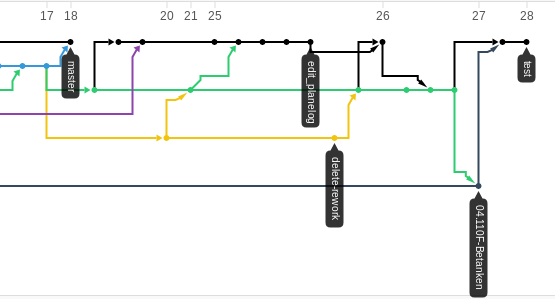
\includegraphics[width=\textwidth]{images/git_network.png}
    \caption{Netzwerk-Graph der Git-Branches}
    \label{fig:git_network}
\end{figure}

\subsection{GitHub}

Die Funktionalität von Git wird erweitert durch Github. Dies bietet die
Möglichkeit, ein zentralen Punkt der Entwicklung zu haben und bringt einige
wichtige \emph{soziale Funktionen} mit sich.

%% PRs
Die wichtigste hierbei ist wohl die \emph{Pull Request}. Dies ist die Bitte an
andere, Änderungen aus dem eigenen Branch in einen anderen Branch zu ziehen.
Ein Beispiel dafür kann sein, dass ein Entwickler ein Feature in einem Branch
entwickelt hat und nun diesen Branch in den Hauptbranch mergen will. Dazu
erstellt er eine Pull Request, und bittet dabei andere Entwickler, seinen Code
zu reviewen. Im Backend wurden insgesamt knapp 20 Pull Requests geöffnet.
 
%% Issues
Neben Pull Requests zur Diskussion über Quellcode gibt es die Möglichkeit, über
\emph{Issues} Fehler zu dokumentieren. die erwies sich insbesondere in den
Kommunikation zwischen den Teams als nützlich.

%% Discord-Bot
Ebenfalls sehr praktisch war der Discord-Bot, der in verschiedenen Kanälen alle nennenswerten Ereignisse im GitHub gepostet hat. So war es motivierten Teilnehmern einfach möglich, die Arbeit der anderen zu verfolgen.

\subsection{Discord}

Discord wurde als zentrale Chat-Plattform genutzt, zum einen, da es die
Möglichkeit gibt, auf einem Server verschiedene Räume für verschiedene Gruppen
zu gestalten und zum anderen, weil einige Teilnehmer Discord bereits beim
Gaming verwenden.

Die Kommunikation über Discord ist insgesamt als positiv zu bewerten, auch wenn
einige Teilnehmer schlecht erreichbar waren oder manche Nachrichten überlesen
wurden.

\subsection{IntelliJ IDEA}

Als \emph{integrierte Entwicklungsumgebung} wurde IntelliJ IDEA genutzt.
IntelliJ bietet etwas mehr Features als Eclipse und ist generell besser
\emph{benutzbar}, da z.~B. schneller.

Besonders hilfreich war die eingebaute Git-Unterstützung, die bei
Merge-Konflikten sehr hilfreich war. Auch die Möglichkeit, sehr einfach Dateien
zu \emph{diffen}, also die Unterschiedlichen Versionen zu vergleichen, war sehr
angenehm.

\subsection{Datenbank}

%% einige H2, andere mysql + dbeaver, mysql-cli
Bei der Datenbank für die lokale Entwicklung gab es verschiedene Ansätze.
Einige Entwickler haben die von Spring automatisch konfigurierte H2-Datenbank
genutzt, die den geringsten (keinen) Einrichtungsaufwand hat. Die Entwickler
mit etwas größerem Interesse an den Ereignissen innerhalb der Datenbank nutzten
lokale MySQL-Instanzen, auf die per HeidiSQL, DBeaver oder per Kommandozeile
zugegriffen wurde.

\subsection{REST-Client}

%% Postman, HTTPie
Zum händischen Testen der definierten Routen wurden \emph{Postman} und
\emph{HTTPie} genutzt. Es war wichtig, die Routen unabhängig vom Frontend selbst
testen zu können, da die Entwicklung so weniger abhängig vom Fortschritt der
Frontendentwicklung war. Dazu wurde insbesondere Postman genutzt. Mit diesem
Tool können HTTP-Anfragen einfach über eine grafische Oberfläche durchgeführt
werden.

Einige nutzten hier stattdessen HTTPie, ein kommandozeilenbasiertes Tool,
welches für schnelle unkomplizierte Abfragen etwas schlanker zu benutzen war.

\subsection{ripgrep}

Eine kurzer aber liebevoller Blick sei noch auf \emph{ripgrep} geworfen, ein
kommandozeilenbasiertes Tool zum durchsuchen von Textdateien per regulären
Ausdrücken \emph{(Regex)}, dass dem UNIX-Programm \emph{grep} ähnelt. Das Tool
wurde zwar nur von einem Entwickler intensiv genutzt, erwies sich aber als
wertvolle Hilfe, um z.~B. alle Vorkommen einer Methode oder einer Annotation im
Projekt zu suchen. 

\end{document}
